\فصل{مقدمات}
\برچسب{فصل:مقدمه}
\قسمت{آغاز مثلاً}
این فصل به مقدمات پایان نامه اختصاص دارد. ابتدا مسأله‌ی ارزیابی کیفیت تصویر(\متن‌لاتین{IQA}\پانویس{Image Quality Assessment}) را تعریف کرده، سپس به کاربردهای آن اشاره می‌کنیم. پس از آن رویکرد نویی که این پایان نامه به مسئله‌ی \متن‌لاتین{IQA} دارد را مورد بررسی قرار داده و نهایتاً ساختار کلی متنی که پیش رو است را از نظر می‌گذرانیم.

\begin{comment}
\begin{figure}[ht]
  \centering
  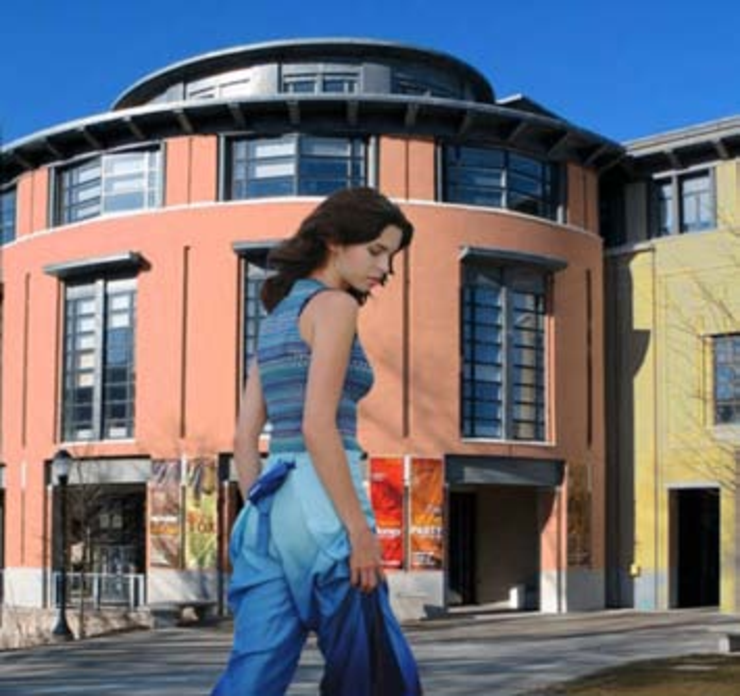
\includegraphics[width=0.9\linewidth]{harmonized.pdf}
  \شرح{شرح \متن‌لاتین{harmonized.pdf} \مرجع{someCitation}}
  \label{شکل:دسته‌های‌IQA}
\end{figure}
\end{comment}
\قسمت{ساختار پایان‌نامه}
